\section{Feed-Forward Neural Network}
In this section, we will discuss how the \class{NeuralNetworkClassifier()} is implemented and how the hyperparameters are chosen, as well as the results of using this model. \\

A feed-forward neural network is a type of artificial neural network that consists of an input layer, one or more hidden layers, and an output layer.
Each layer consists of a set of neurons, which are connected to the neurons in the next layer through weights.
The input layer receives input data and passes it through the network to the output layer, where the output is produced. \\

The hidden layers process the input data and transform it into a form that can be used by the output layer to produce a prediction.
The weights of the connections between neurons are adjusted during the training process to minimize the difference between the predicted output and the actual output, a process known as backpropagation. \\

Feed-forward neural networks can be used for a wide range of tasks, including image and speech recognition, natural language processing, and predicting outcomes in complex systems.
They are a popular choice for machine learning tasks due to their ability to learn and generalize from data.
Typically neural networks require significantly more training-data than the traditional machine learning methods to produce desirable results. \\

\begin{figure}[H]
    \centering
    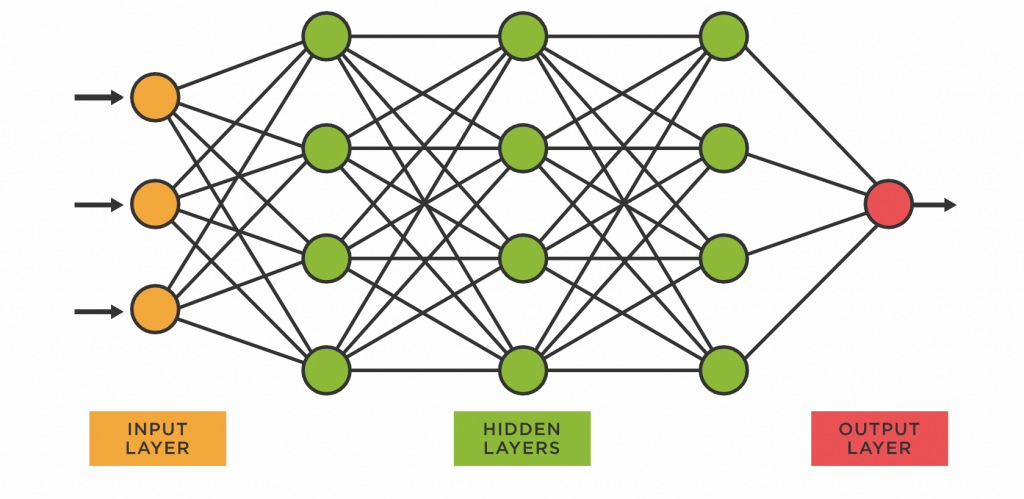
\includegraphics[scale=0.3]{figures_for_report/simple_neural_network}
    \captionsetup{justification=centering,margin=2cm}
    \caption{A Simple Neural Network Architecture}
\end{figure}


\subsection{Implementation}
The implementation of the Feed-Forward Neural Network was done in Python using two classes. \\
\begin{enumerate}
    \item \class{DenseLayer()}
    \item \class{NeuralNetworkClassifier()}
    \end{enumerate}
\vspace{10pt}

\subsubsection{DenseLayer()}
The \class{DenseLayer()} represents the hidden-layers and the output layer that make up the network.
It should be initialized with a \code{layer_size} and an \code{activation}.
The \code{layer_size} represents the number of neurons in the layer, for example
if you have a multiclass classification with 3 classes the output layer should have \code{layer_size=3}.
The \code{activation} parameter is the activation function to be applied to the output of the layer.
The current implemented activation-functions are Sigmoid, ReLU and Softmax, where Softmax can only be applied to the output layer.\\

The \class{DenseLayer()} has two primary methods \code{forward()} and \code{backward()}.
The \code{forward(x, weights, bias)} method performs a forward pass through the layer, given the input data (\code{x}), weights (\code{weights}), and biases (\code{bias}).
It calculates the dot product of the inputs and weights, adds the bias, and applies the activation function to the result to produce the output of the layer.
It returns the pre-activated output of the layer, and the activation of the layer.
The \code{backward(dA_curr, W_curr, Z_curr, A_prev)} method performs the backward pass through the layer, given the gradient of the cost with respect to the current layer's activations \code{(dA_curr)}, the current layer's weights \code{(W_curr)}, the current layer's pre-activation values \code{(Z_curr)}, and the previous layer's activations (\code{A_prev}).
It calculates the gradients of the cost with respect to the weights (\code{dW}), biases (\code{db)}, and previous layer's activations (\code{dA}) using the chain rule.
The return values of both the \code{forward()} and the \code{backward()} method are needed for backpropagation which happens in the \class{NeuralNetworkClassifier()}.


\subsubsection{NeuralNetworkClassifier()}
The \class{NeuralNetworkClassifier()} is the classifier class.
It's primary methods are \code{fit()} and \code{predict()}.
Additionally, it includes a lot of helper methods that all have different responsibilities.
These include initializing and updating weights and biases based on the layer sizes and input data dimensions specified.
The constructor take the following four parameters:\\
\begin{itemize}
    \item \code{layers} - (A list of DenseLayer objects - the layers in the network)
    \item \code{learning_rate} - (A float - how fast the weights update after each mini-batch)
    \item \code{epochs} - (An integer - the number of epochs to train the neural network for)
    \item \code{random_state} - (An integer - set the random seed for reproducible results)
    \end{itemize}
\vspace{10pt}


The \code{fit(X, y, batch_size, validation_size)} method is used to train the model, and takes four parameters:
The training data (\code{X}) and labels (\code{y}), the \code{batch_size} (an integer indicating the number of samples to use in each mini-batch during training).
Lastly \code{validation_size} (a float indicating the proportion of the training data to use for validation).
To keep it short the \code{fit()} method does the following:
For each mini-batch, the model makes predictions using the \code{_forward()} method, computes the loss using the \code{delta_cross_entropy()} function.
It then performs backpropagation with the \code{_backward()} method and finally updates weights and biases using the gradients calculated with the \code{_backward()} method.
This process is performed as many times as specified with by the \code{epoch} parameter in the constructor.

\subsection{Correctness}
For the scope of this project the correctness of our implementation was done primarily visually.
The training accuracy and training loss was compared to a similar model from the TensorFlow library.
The models used have two ReLU activated hidden layers with 128 and 64 neurons respectively, a Softmax activated output layer with 5 neurons (one for each clothing type) and a learning rate of $0.01$.
For reproduction of these exact graphs \code{random_state=42}, and \code{tf.random.set_seed(42)} should be used. \\

\begin{figure}[H]
    \centering
    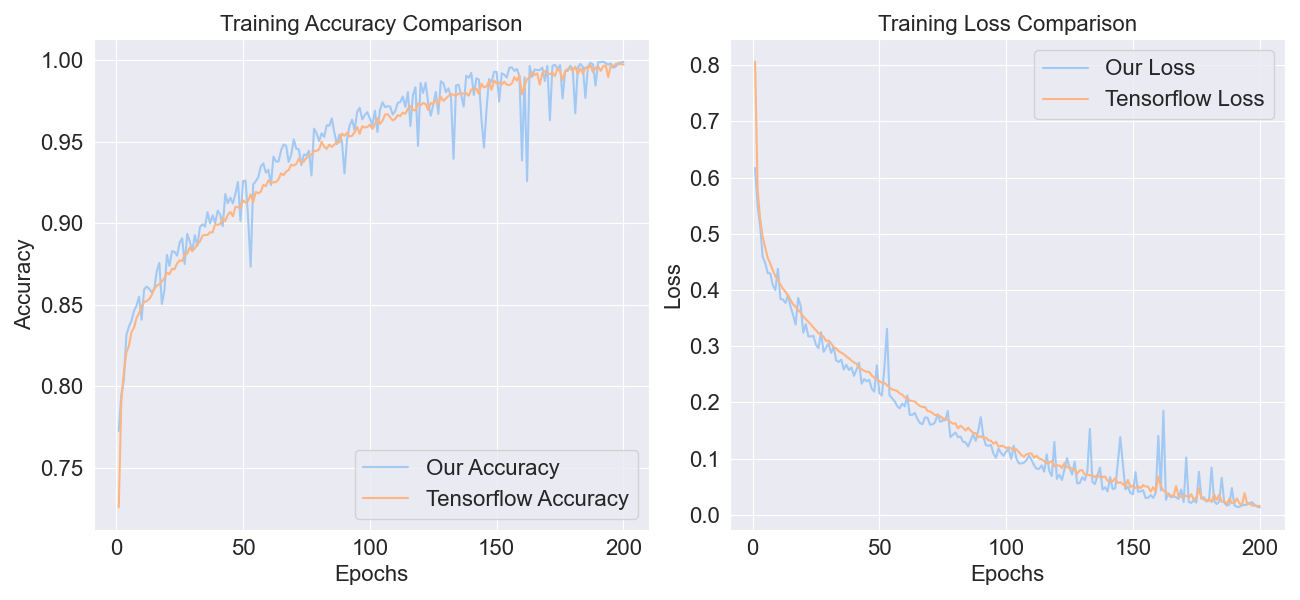
\includegraphics[scale=0.45]{figures_for_report/tensorflow_vs_our}
    \captionsetup{justification=centering,margin=2cm}
    \caption{Comparing Accuracy and Loss with TensorFlow}
\end{figure}

The trend in accuracy and loss for our model, as shown in \textbf{Figure 7}, is comparable to that of TensorFlow's model.
However, TensorFlow's model exhibits a smoother trend in the curves, due to its better optimization.
Based on the results displayed in \textbf{Figure 7}, our model can be considered to have been implemented correctly.

\subsection{Hyperparameters}
Neural networks are known for their ability to learn and generalize from data.
However, they can sometimes suffer from overfitting if the number of epochs or learning rate is set too high.
When selecting a good set of hyperparameters, we focused solely on the number of epochs and kept all other parameters fixed, including the hidden layers and other parameters mentioned in section 5\textbf{5.2}, and the following parameters as well \code{learning_rate=0.01}, \code{batch_size=32}, \code{random_state=42}.
To reduce overfitting, it was optimal to choose a number of epochs that resulted in a high validation accuracy and low validation loss
\textbf{Figure 8} shows the models performance during training and was used to choose $70$ as the number of epochs.
These parameters were then used to train an instance of the \class{NeuralNetworkClassifier()} and the results are reported in the following section.
\begin{figure}[H]
    \centering
    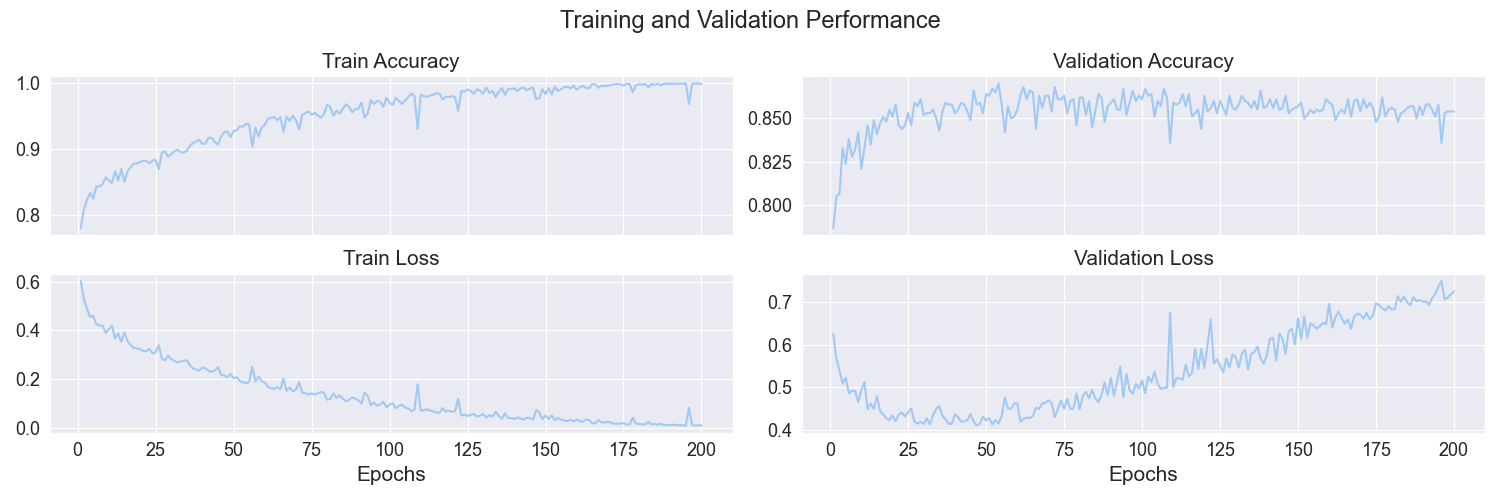
\includegraphics[scale=0.45]{figures_for_report/train_validation_nn_performance}
    \captionsetup{justification=centering,margin=2cm}
    \caption{Performance during training}\label{fig:figure}
\end{figure}

\subsection{Results}\label{subsec:results}
\begin{table}[!ht]
\begin{subtable}[c]{0.4\textwidth}
\footnotesize
\centering
\begin{tabular}{ c | c }
 \toprule
 Evaluation Metric & Accuracy Score  \\
 \midrule
 Training Accuracy & 94.43\% \\
 Test Accuracy & 85.20\% \\
 \bottomrule
\end{tabular}
\captionsetup{justification=centering,margin=1cm}
\end{subtable}
\begin{subtable}[c]{0.6\textwidth}
\footnotesize
\centering
\begin{tabular}{c | c c r}
Class & Precision & Recall & F1-Score\\
\midrule
T-shirt/Top   &    0.81  &    0.82  &    0.82 \\
Trousers   &    0.98  &    0.97  &    0.98 \\
Pullover   &    0.86  &    0.84  &    0.85\\
Dress   &    0.90  &    0.90  &    0.90\\
Shirt   &    0.72  &    0.73  &    0.73\\
\end{tabular}
\captionsetup{justification=centering,margin=1cm}
\end{subtable}
\caption{Neural Network Performance}
\label{nn_evaluation}
\end{table}\\

The \class{NeuralNetworkClassifier()} achieved a test accuracy of $85.16\%$ and training accuracy of $94.29\%$.
Again, our model emphasizes the difficulties in correctly classifying shirts, as seen by the Precision, Recall and F1-score in \textbf{Table 3}.
The model performs well on correctly classifying Trousers and Dresses, with an achieved F1-score of 0.97 and 0.9.







